\documentclass{standalone}
\usepackage{tikz}
\usetikzlibrary{patterns, positioning}

\begin{document}
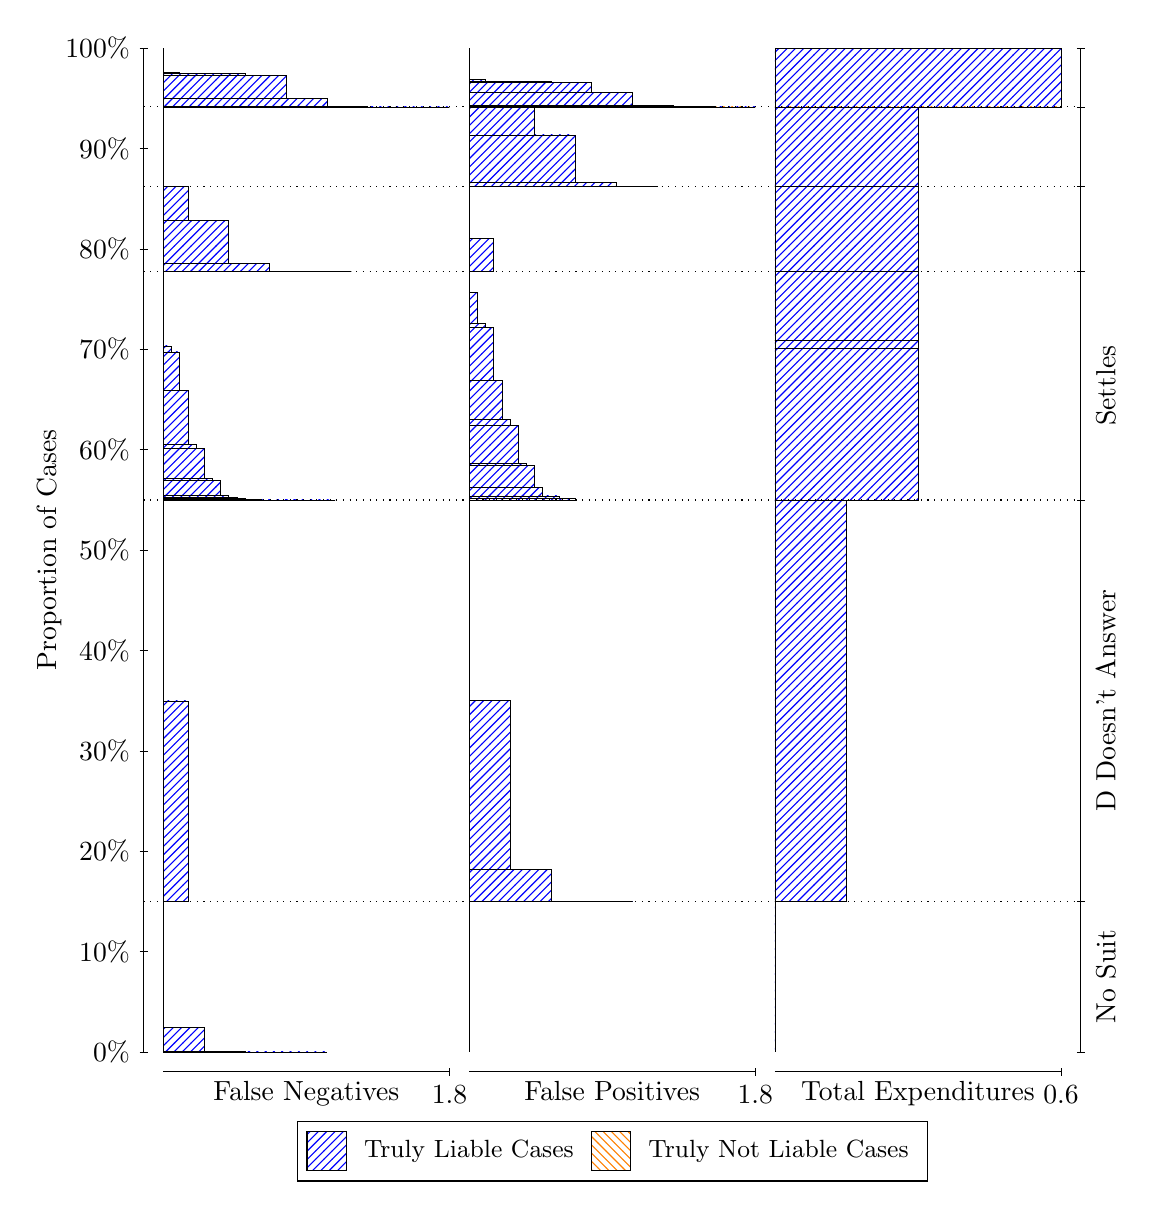
\begin{tikzpicture}
\draw[black, very thin] (1.5,1.75) -- (1.5,14.5);
\node[rotate=90, anchor=center] at (0.3, 8.125) {Proportion of Cases};
\draw[black, very thin] (1.45,1.75) -- (1.55,1.75);
\node[anchor=east] at (1.45, 1.75) {0\%};
\draw[black, very thin] (1.45,3.025) -- (1.55,3.025);
\node[anchor=east] at (1.45, 3.025) {10\%};
\draw[black, very thin] (1.45,4.3) -- (1.55,4.3);
\node[anchor=east] at (1.45, 4.3) {20\%};
\draw[black, very thin] (1.45,5.575) -- (1.55,5.575);
\node[anchor=east] at (1.45, 5.575) {30\%};
\draw[black, very thin] (1.45,6.85) -- (1.55,6.85);
\node[anchor=east] at (1.45, 6.85) {40\%};
\draw[black, very thin] (1.45,8.125) -- (1.55,8.125);
\node[anchor=east] at (1.45, 8.125) {50\%};
\draw[black, very thin] (1.45,9.4) -- (1.55,9.4);
\node[anchor=east] at (1.45, 9.4) {60\%};
\draw[black, very thin] (1.45,10.675) -- (1.55,10.675);
\node[anchor=east] at (1.45, 10.675) {70\%};
\draw[black, very thin] (1.45,11.95) -- (1.55,11.95);
\node[anchor=east] at (1.45, 11.95) {80\%};
\draw[black, very thin] (1.45,13.225) -- (1.55,13.225);
\node[anchor=east] at (1.45, 13.225) {90\%};
\draw[black, very thin] (1.45,14.5) -- (1.55,14.5);
\node[anchor=east] at (1.45, 14.5) {100\%};

\draw[black, very thin] (13.4,1.75) -- (13.4,14.5);
\draw[black, very thin] (13.35,1.75) -- (13.45,1.75);
\node[anchor=west] at (13.35, 1.75) {};
\draw[black, very thin] (13.35,3.6628) -- (13.45,3.6628);
\node[anchor=west] at (13.35, 3.6628) {};
\draw[black, very thin] (13.35,8.7607) -- (13.45,8.7607);
\node[anchor=west] at (13.35, 8.7607) {};
\draw[black, very thin] (13.35,11.662) -- (13.45,11.662);
\node[anchor=west] at (13.35, 11.662) {};
\draw[black, very thin] (13.35,12.739) -- (13.45,12.739);
\node[anchor=west] at (13.35, 12.739) {};
\draw[black, very thin] (13.35,13.753) -- (13.45,13.753);
\node[anchor=west] at (13.35, 13.753) {};
\draw[black, very thin] (13.35,14.5) -- (13.45,14.5);
\node[anchor=west] at (13.35, 14.5) {};

\draw[black, very thin, pattern color=blue, pattern=north east lines] (1.75,1.75) rectangle (3.8262,1.75);
\draw[black, very thin, pattern color=blue, pattern=north east lines] (1.75,1.75) rectangle (3.3071,1.75);
\draw[black, very thin, pattern color=blue, pattern=north east lines] (1.75,1.75) rectangle (2.7881,1.7527);
\draw[black, very thin, pattern color=blue, pattern=north east lines] (1.75,1.7527) rectangle (2.269,2.0632);
\draw[black, very thin, pattern color=orange, pattern=north west lines] (1.75,2.0632) rectangle (1.75,2.0632);
\draw[black, very thin, pattern color=blue, pattern=north east lines] (1.75,2.0632) rectangle (1.75,3.6628);
\draw[black, very thin, pattern color=blue, pattern=north east lines] (1.75,3.6628) rectangle (2.0614,6.2086);
\draw[black, very thin, pattern color=orange, pattern=north west lines] (1.75,6.2086) rectangle (1.75,6.2086);
\draw[black, very thin, pattern color=blue, pattern=north east lines] (1.75,6.2086) rectangle (1.75,8.7607);
\draw[black, very thin, pattern color=blue, pattern=north east lines] (1.75,8.7607) rectangle (3.93,8.7607);
\draw[black, very thin, pattern color=blue, pattern=north east lines] (1.75,8.7607) rectangle (3.7224,8.7607);
\draw[black, very thin, pattern color=blue, pattern=north east lines] (1.75,8.7607) rectangle (3.5148,8.7607);
\draw[black, very thin, pattern color=blue, pattern=north east lines] (1.75,8.7607) rectangle (3.411,8.7607);
\draw[black, very thin, pattern color=blue, pattern=north east lines] (1.75,8.7607) rectangle (3.3071,8.7607);
\draw[black, very thin, pattern color=blue, pattern=north east lines] (1.75,8.7607) rectangle (3.2033,8.7609);
\draw[black, very thin, pattern color=blue, pattern=north east lines] (1.75,8.7609) rectangle (3.0995,8.7609);
\draw[black, very thin, pattern color=blue, pattern=north east lines] (1.75,8.7609) rectangle (2.9957,8.7654);
\draw[black, very thin, pattern color=blue, pattern=north east lines] (1.75,8.7654) rectangle (2.8919,8.7662);
\draw[black, very thin, pattern color=blue, pattern=north east lines] (1.75,8.7662) rectangle (2.7881,8.7782);
\draw[black, very thin, pattern color=blue, pattern=north east lines] (1.75,8.7782) rectangle (2.6843,8.7895);
\draw[black, very thin, pattern color=blue, pattern=north east lines] (1.75,8.7895) rectangle (2.5805,8.8192);
\draw[black, very thin, pattern color=blue, pattern=north east lines] (1.75,8.8192) rectangle (2.4767,9.0046);
\draw[black, very thin, pattern color=blue, pattern=north east lines] (1.75,9.0046) rectangle (2.3729,9.0304);
\draw[black, very thin, pattern color=blue, pattern=north east lines] (1.75,9.0304) rectangle (2.269,9.4173);
\draw[black, very thin, pattern color=blue, pattern=north east lines] (1.75,9.4173) rectangle (2.1652,9.467);
\draw[black, very thin, pattern color=blue, pattern=north east lines] (1.75,9.467) rectangle (2.0614,10.148);
\draw[black, very thin, pattern color=blue, pattern=north east lines] (1.75,10.148) rectangle (1.9576,10.64);
\draw[black, very thin, pattern color=blue, pattern=north east lines] (1.75,10.64) rectangle (1.8538,10.718);
\draw[black, very thin, pattern color=orange, pattern=north west lines] (1.75,10.718) rectangle (1.75,10.718);
\draw[black, very thin, pattern color=blue, pattern=north east lines] (1.75,10.718) rectangle (1.75,11.662);
\draw[black, very thin, pattern color=blue, pattern=north east lines] (1.75,11.662) rectangle (4.1376,11.662);
\draw[black, very thin, pattern color=blue, pattern=north east lines] (1.75,11.662) rectangle (3.6186,11.664);
\draw[black, very thin, pattern color=blue, pattern=north east lines] (1.75,11.664) rectangle (3.0995,11.765);
\draw[black, very thin, pattern color=blue, pattern=north east lines] (1.75,11.765) rectangle (2.5805,12.315);
\draw[black, very thin, pattern color=blue, pattern=north east lines] (1.75,12.315) rectangle (2.0614,12.739);
\draw[black, very thin, pattern color=orange, pattern=north west lines] (1.75,12.739) rectangle (1.75,12.739);
\draw[black, very thin, pattern color=blue, pattern=north east lines] (1.75,12.739) rectangle (2.0614,12.743);
\draw[black, very thin, pattern color=orange, pattern=north west lines] (1.75,12.743) rectangle (1.75,12.743);
\draw[black, very thin, pattern color=blue, pattern=north east lines] (1.75,12.743) rectangle (1.75,13.753);
\draw[black, very thin, pattern color=blue, pattern=north east lines] (1.75,13.753) rectangle (5.3833,13.753);
\draw[black, very thin, pattern color=blue, pattern=north east lines] (1.75,13.753) rectangle (4.8643,13.753);
\draw[black, very thin, pattern color=blue, pattern=north east lines] (1.75,13.753) rectangle (4.3452,13.757);
\draw[black, very thin, pattern color=blue, pattern=north east lines] (1.75,13.757) rectangle (3.8262,13.863);
\draw[black, very thin, pattern color=blue, pattern=north east lines] (1.75,13.863) rectangle (3.3071,14.153);
\draw[black, very thin, pattern color=blue, pattern=north east lines] (1.75,14.153) rectangle (2.9957,14.153);
\draw[black, very thin, pattern color=blue, pattern=north east lines] (1.75,14.153) rectangle (2.7881,14.179);
\draw[black, very thin, pattern color=blue, pattern=north east lines] (1.75,14.179) rectangle (2.4767,14.179);
\draw[black, very thin, pattern color=blue, pattern=north east lines] (1.75,14.179) rectangle (2.4767,14.179);
\draw[black, very thin, pattern color=blue, pattern=north east lines] (1.75,14.179) rectangle (2.269,14.18);
\draw[black, very thin, pattern color=blue, pattern=north east lines] (1.75,14.18) rectangle (1.9576,14.18);
\draw[black, very thin, pattern color=blue, pattern=north east lines] (1.75,14.18) rectangle (1.9576,14.187);
\draw[black, very thin, pattern color=orange, pattern=north west lines] (1.75,14.187) rectangle (1.75,14.187);
\draw[black, very thin, pattern color=blue, pattern=north east lines] (1.75,14.187) rectangle (1.75,14.5);
\draw[black, very thin, pattern color=orange, pattern=north west lines] (5.6333,1.75) rectangle (5.6333,1.75);
\draw[black, very thin, pattern color=blue, pattern=north east lines] (5.6333,1.75) rectangle (5.6333,3.6628);
\draw[black, very thin, pattern color=orange, pattern=north west lines] (5.6333,3.6628) rectangle (7.7095,3.6628);
\draw[black, very thin, pattern color=blue, pattern=north east lines] (5.6333,3.6628) rectangle (7.7095,3.6628);
\draw[black, very thin, pattern color=blue, pattern=north east lines] (5.6333,3.6628) rectangle (7.1905,3.6658);
\draw[black, very thin, pattern color=blue, pattern=north east lines] (5.6333,3.6658) rectangle (6.6714,4.0699);
\draw[black, very thin, pattern color=blue, pattern=north east lines] (5.6333,4.0699) rectangle (6.1524,6.2149);
\draw[black, very thin, pattern color=blue, pattern=north east lines] (5.6333,6.2149) rectangle (5.6333,8.7607);
\draw[black, very thin, pattern color=orange, pattern=north west lines] (5.6333,8.7607) rectangle (6.9829,8.7607);
\draw[black, very thin, pattern color=blue, pattern=north east lines] (5.6333,8.7607) rectangle (6.9829,8.7768);
\draw[black, very thin, pattern color=orange, pattern=north west lines] (5.6333,8.7768) rectangle (6.7752,8.7768);
\draw[black, very thin, pattern color=blue, pattern=north east lines] (5.6333,8.7768) rectangle (6.7752,8.8119);
\draw[black, very thin, pattern color=orange, pattern=north west lines] (5.6333,8.8119) rectangle (6.5676,8.8119);
\draw[black, very thin, pattern color=blue, pattern=north east lines] (5.6333,8.8119) rectangle (6.5676,8.9191);
\draw[black, very thin, pattern color=blue, pattern=north east lines] (5.6333,8.9191) rectangle (6.4638,9.1969);
\draw[black, very thin, pattern color=orange, pattern=north west lines] (5.6333,9.1969) rectangle (6.36,9.1969);
\draw[black, very thin, pattern color=blue, pattern=north east lines] (5.6333,9.1969) rectangle (6.36,9.2231);
\draw[black, very thin, pattern color=blue, pattern=north east lines] (5.6333,9.2231) rectangle (6.2562,9.7048);
\draw[black, very thin, pattern color=orange, pattern=north west lines] (5.6333,9.7048) rectangle (6.1524,9.7048);
\draw[black, very thin, pattern color=blue, pattern=north east lines] (5.6333,9.7048) rectangle (6.1524,9.7823);
\draw[black, very thin, pattern color=blue, pattern=north east lines] (5.6333,9.7823) rectangle (6.0486,10.275);
\draw[black, very thin, pattern color=blue, pattern=north east lines] (5.6333,10.275) rectangle (5.9448,10.956);
\draw[black, very thin, pattern color=blue, pattern=north east lines] (5.6333,10.956) rectangle (5.841,11.005);
\draw[black, very thin, pattern color=blue, pattern=north east lines] (5.6333,11.005) rectangle (5.7371,11.392);
\draw[black, very thin, pattern color=blue, pattern=north east lines] (5.6333,11.392) rectangle (5.6333,11.662);
\draw[black, very thin, pattern color=orange, pattern=north west lines] (5.6333,11.662) rectangle (5.9448,11.662);
\draw[black, very thin, pattern color=blue, pattern=north east lines] (5.6333,11.662) rectangle (5.9448,12.086);
\draw[black, very thin, pattern color=blue, pattern=north east lines] (5.6333,12.086) rectangle (5.6333,12.739);
\draw[black, very thin, pattern color=orange, pattern=north west lines] (5.6333,12.739) rectangle (8.021,12.739);
\draw[black, very thin, pattern color=blue, pattern=north east lines] (5.6333,12.739) rectangle (8.021,12.74);
\draw[black, very thin, pattern color=blue, pattern=north east lines] (5.6333,12.74) rectangle (7.5019,12.793);
\draw[black, very thin, pattern color=blue, pattern=north east lines] (5.6333,12.793) rectangle (6.9829,13.396);
\draw[black, very thin, pattern color=blue, pattern=north east lines] (5.6333,13.396) rectangle (6.4638,13.749);
\draw[black, very thin, pattern color=blue, pattern=north east lines] (5.6333,13.749) rectangle (5.9448,13.753);
\draw[black, very thin, pattern color=orange, pattern=north west lines] (5.6333,13.753) rectangle (9.2667,13.753);
\draw[black, very thin, pattern color=blue, pattern=north east lines] (5.6333,13.753) rectangle (9.2667,13.753);
\draw[black, very thin, pattern color=orange, pattern=north west lines] (5.6333,13.753) rectangle (8.7476,13.753);
\draw[black, very thin, pattern color=blue, pattern=north east lines] (5.6333,13.753) rectangle (8.7476,13.754);
\draw[black, very thin, pattern color=orange, pattern=north west lines] (5.6333,13.754) rectangle (8.2286,13.754);
\draw[black, very thin, pattern color=blue, pattern=north east lines] (5.6333,13.754) rectangle (8.2286,13.772);
\draw[black, very thin, pattern color=orange, pattern=north west lines] (5.6333,13.772) rectangle (7.7095,13.772);
\draw[black, very thin, pattern color=blue, pattern=north east lines] (5.6333,13.772) rectangle (7.7095,13.939);
\draw[black, very thin, pattern color=blue, pattern=north east lines] (5.6333,13.939) rectangle (7.1905,14.066);
\draw[black, very thin, pattern color=blue, pattern=north east lines] (5.6333,14.066) rectangle (6.6714,14.074);
\draw[black, very thin, pattern color=orange, pattern=north west lines] (5.6333,14.074) rectangle (6.36,14.074);
\draw[black, very thin, pattern color=blue, pattern=north east lines] (5.6333,14.074) rectangle (6.36,14.074);
\draw[black, very thin, pattern color=blue, pattern=north east lines] (5.6333,14.074) rectangle (6.1524,14.074);
\draw[black, very thin, pattern color=orange, pattern=north west lines] (5.6333,14.074) rectangle (5.841,14.074);
\draw[black, very thin, pattern color=blue, pattern=north east lines] (5.6333,14.074) rectangle (5.841,14.101);
\draw[black, very thin, pattern color=orange, pattern=north west lines] (5.6333,14.101) rectangle (5.6333,14.101);
\draw[black, very thin, pattern color=blue, pattern=north east lines] (5.6333,14.101) rectangle (5.6333,14.5);
\draw[black, very thin, pattern color=orange, pattern=north west lines] (9.5167,1.75) rectangle (9.5167,1.75);
\draw[black, very thin, pattern color=blue, pattern=north east lines] (9.5167,1.75) rectangle (9.5167,3.6628);
\draw[black, very thin, pattern color=orange, pattern=north west lines] (9.5167,3.6628) rectangle (10.425,3.6628);
\draw[black, very thin, pattern color=blue, pattern=north east lines] (9.5167,3.6628) rectangle (10.425,8.7607);
\draw[black, very thin, pattern color=orange, pattern=north west lines] (9.5167,8.7607) rectangle (11.333,8.7607);
\draw[black, very thin, pattern color=blue, pattern=north east lines] (9.5167,8.7607) rectangle (11.333,10.681);
\draw[black, very thin, pattern color=orange, pattern=north west lines] (9.5167,10.681) rectangle (11.333,10.681);
\draw[black, very thin, pattern color=blue, pattern=north east lines] (9.5167,10.681) rectangle (11.333,10.785);
\draw[black, very thin, pattern color=orange, pattern=north west lines] (9.5167,10.785) rectangle (11.333,10.785);
\draw[black, very thin, pattern color=blue, pattern=north east lines] (9.5167,10.785) rectangle (11.333,11.662);
\draw[black, very thin, pattern color=orange, pattern=north west lines] (9.5167,11.662) rectangle (11.333,11.662);
\draw[black, very thin, pattern color=blue, pattern=north east lines] (9.5167,11.662) rectangle (11.333,12.739);
\draw[black, very thin, pattern color=orange, pattern=north west lines] (9.5167,12.739) rectangle (11.333,12.739);
\draw[black, very thin, pattern color=blue, pattern=north east lines] (9.5167,12.739) rectangle (11.333,13.753);
\draw[black, very thin, pattern color=orange, pattern=north west lines] (9.5167,13.753) rectangle (13.15,13.753);
\draw[black, very thin, pattern color=blue, pattern=north east lines] (9.5167,13.753) rectangle (13.15,14.5);
\draw[black, dotted] (1.5,3.6628) -- (13.4,3.6628);
\draw[black, dotted] (1.5,8.7607) -- (13.4,8.7607);
\draw[black, dotted] (1.5,11.662) -- (13.4,11.662);
\draw[black, dotted] (1.5,12.739) -- (13.4,12.739);
\draw[black, dotted] (1.5,13.753) -- (13.4,13.753);
\draw[black, very thin] (1.75,1.5) -- (5.3833,1.5);
\node[anchor=north] at (3.5667, 1.5) {False Negatives};
\draw[black, very thin] (5.3833,1.45) -- (5.3833,1.55);
\node[anchor=north] at (5.3833, 1.45) {1.8};

\draw[black, very thin] (5.6333,1.5) -- (9.2667,1.5);
\node[anchor=north] at (7.45, 1.5) {False Positives};
\draw[black, very thin] (9.2667,1.45) -- (9.2667,1.55);
\node[anchor=north] at (9.2667, 1.45) {1.8};

\draw[black, very thin] (9.5167,1.5) -- (13.15,1.5);
\node[anchor=north] at (11.333, 1.5) {Total Expenditures};
\draw[black, very thin] (13.15,1.45) -- (13.15,1.55);
\node[anchor=north] at (13.15, 1.45) {0.6};

\node[black, centered, rotate=90] at (13.72, 2.7064) {No Suit};
\node[black, centered, rotate=90] at (13.72, 6.2117) {D Doesn't Answer};
\node[black, centered, rotate=90] at (13.72, 10.211) {Settles};




\draw (7.449999999999999,1.5) node[draw=none] (baseCoordinate) {};
\begin{scope}[align=center]
        \matrix[scale=0.5, draw=black, below=0.5cm of baseCoordinate, nodes={draw}, column sep=0.1cm]{
            \node[rectangle, draw, minimum width=0.5cm, minimum height=0.5cm, pattern=north east lines, pattern color=blue] {}; &
            \node[draw=none, font=\small] (B) {Truly Liable Cases}; &
            \node[rectangle, draw, minimum width=0.5cm, minimum height=0.5cm, pattern=north west lines, pattern color=orange] {}; &
            \node[draw=none, font=\small] (B) {Truly Not Liable Cases}; \\
            };
\end{scope}

\end{tikzpicture}
\end{document}